\documentclass[aspectratio=169, t]{beamer}

\usetheme{metropolis}

% RUB Farben definieren
\definecolor{rub-blue}{RGB}{0,53,96}
\definecolor{rub-green}{RGB}{141,174,16}
\definecolor{rub-grey}{RGB}{231,231,231}

% Metropolis Farbschema anpassen
\setbeamercolor{normal text}{fg=rub-blue!90!black, bg=white}
\setbeamercolor{alerted text}{fg=rub-green}
\setbeamercolor{frametitle}{bg=rub-blue, fg=white}
\setbeamercolor{progress bar}{fg=rub-green, bg=rub-grey}
\setbeamercolor{title separator}{fg=rub-green}
% palette primary steuert Section- und Titelfolien in Metropolis
\setbeamercolor{palette primary}{bg=rub-blue, fg=white}

\metroset{
    progressbar=frametitle,
    block=fill,
    numbering=fraction
}

\usepackage[utf8]{inputenc}
\usepackage[T1]{fontenc}
\usepackage{lmodern}
\usepackage{microtype}
\usepackage{hyperref}

% Inline-Code-Befehl mit sichtbarem grauem Hintergrund
% \bt erzeugt einen Backtick (Gravis) in T1-Kodierung
\newcommand{\bt}{\textasciigrave}
\newcommand{\icode}[1]{%
    \begingroup
    \setlength\fboxsep{2.5pt}%
    \colorbox{rub-grey}{\texttt{\color{rub-blue}\small\strut #1}}%
    \endgroup
}

\title{CTM Workshop for Quarto}
\subtitle{Lund 2026}
\author{Noah Wolfs-Gäer \& Michael Kallweit}
\institute{Ruhr University Bochum}
\date{19.03.2026}

\begin{document}

\maketitle

\begin{frame}{Introduction}
    \begin{itemize}
        \item First of all, thank you for inviting us to Lund.
        \item Today, we would like to present Quarto to you.
        \item (Most of you probably already know it.)
        \item For those who are new to Quarto, this presentation features a beginner's guide.
    \end{itemize}
\end{frame}

\begin{frame}{Table of contents}
    \tableofcontents
\end{frame}

\section{For Beginners}

\begin{frame}{What is Quarto?}
    \begin{itemize}
        \item Website: \url{https://quarto.org/}
        \item You write standard Markdown code exactly how you want it to appear.
        \item You can also embed code (Python, R, Julia, Observable, \dots).
        \item During rendering, Quarto scans the file for code blocks. Each code block is processed by the appropriate engine, and the output is inserted into the document.
        \item Quarto then uses Pandoc to format the page using Bootstrap themes.
        \item Finally, it generates an HTML web page, or if you want other formats such as PDF, .docx, \dots
    \end{itemize}
\end{frame}

\begin{frame}{How we use it}
    \begin{itemize}
        \item We currently use it to demonstrate how Python can illustrate basic mathematics (like curve analysis) or help visualize matrix transformations.
        \item For this, we create website projects that include ``pyodide-python'', a web-based Python environment allowing users to run code without local installation.
        \item Michael and others expanded a pyodide-python extension to include AI feedback. Michael can probably explain the technical details.
        \item Quarto can also be used for interactive learning sessions, including quizzes.
    \end{itemize}
\end{frame}

\begin{frame}{How to get started with Quarto}
    \begin{columns}[c]
        \begin{column}{0.6\textwidth}
            \begin{itemize}
                \item Install an IDE of your choice (any text editor works).
                \item For this guide, we use Visual Studio Code.
                \item Install VSCode: \url{https://code.visualstudio.com/download}
                \item Install Quarto: \url{https://quarto.org/docs/get-started/}
                \item Then, install the Quarto extension for VSCode.
                \item Click the icon in the bottom left to find extensions.
            \end{itemize}
        \end{column}
        \begin{column}{0.4\textwidth}
            \fbox{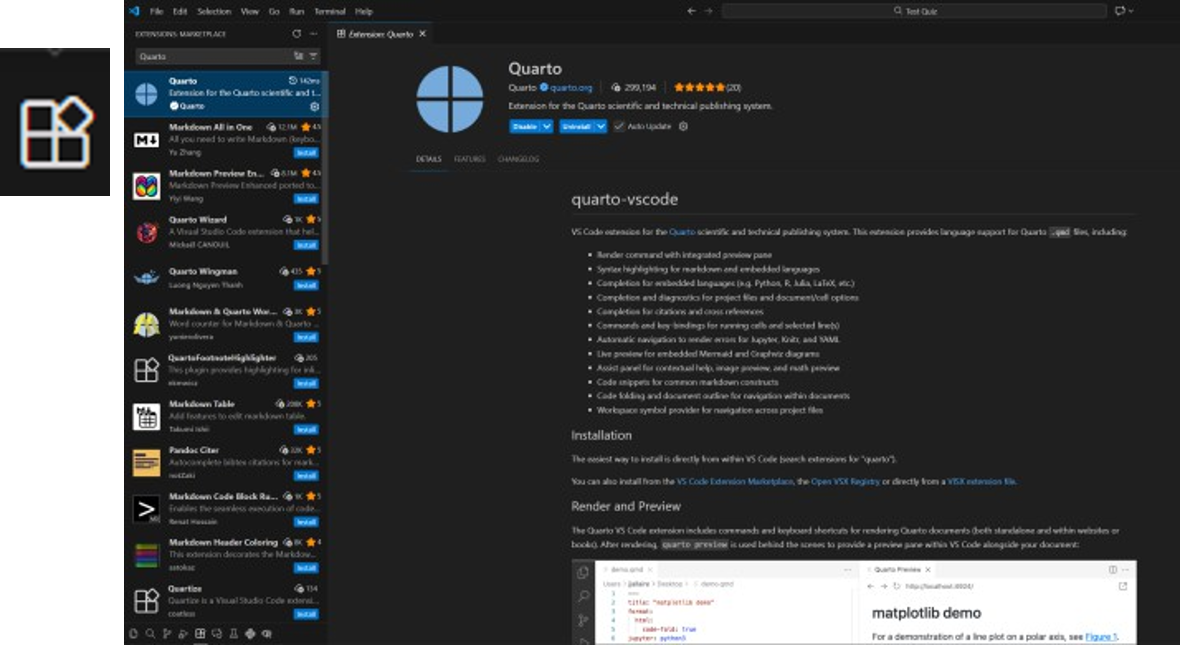
\includegraphics[width=\textwidth]{Images/vscode_extensions.png}}
        \end{column}
    \end{columns}
\end{frame}

\begin{frame}{Getting to know Quarto (in VSCode)}
    \begin{columns}[c]
        \begin{column}{0.6\textwidth}
            \begin{itemize}
                \item Go to File $\rightarrow$ New File
                \item When creating a new Quarto project, the following prompt should appear:
                \item Here, we select 'Website Project', as that fits our needs.
            \end{itemize}
        \end{column}
        \begin{column}{0.4\textwidth}
            \fbox{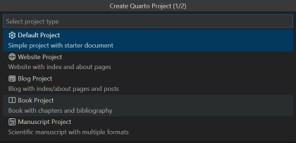
\includegraphics[width=\textwidth]{Images/website_project.png}}
        \end{column}
    \end{columns}
\end{frame}

\begin{frame}{Getting to know Quarto (in VSCode)}
    \begin{columns}[c]
        \begin{column}{0.6\textwidth}
            \begin{itemize}
                \item You should now have 4 files: \icode{\_quarto.yml}, \icode{about.qmd}, \icode{index.qmd}, \icode{styles.css}
                \item These files form the foundation of a Quarto website. You can already render and preview the site (via the terminal with \icode{quarto render} or the render button in the top right of any .qmd file).
                \item The \icode{\_quarto.yml} is the configuration file for the website; here you can adjust the core design and global settings.
                \item Each .qmd file has a YAML header (marked by \icode{---} at the top and bottom). Here you can override settings for that specific page.
            \end{itemize}
        \end{column}
        \begin{column}{0.4\textwidth}
            \fbox{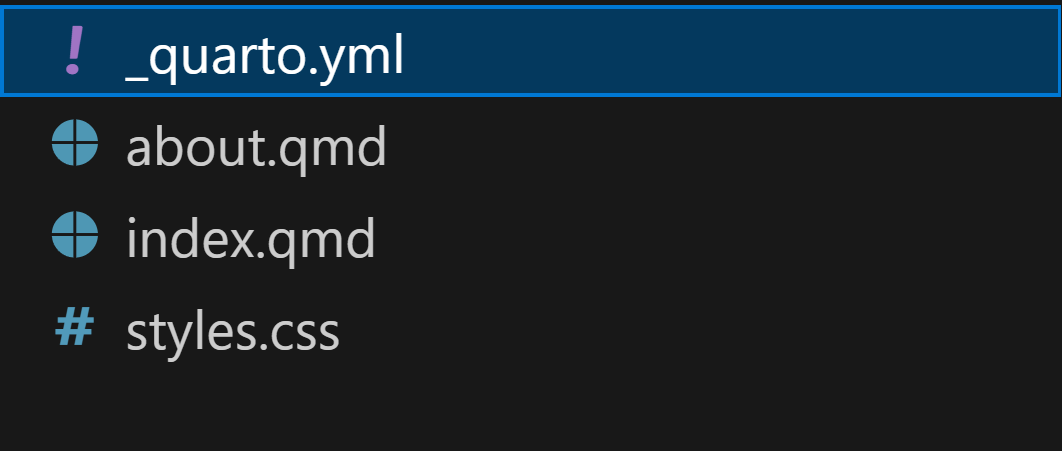
\includegraphics[width=\textwidth]{Images/4_base_files.png}}
        \end{column}
    \end{columns}
\end{frame}

\begin{frame}{Quarto-Syntax}
    \begin{itemize}
        \item \icode{\#, \#\#, \#\#\#} creates sections, subsections, subsubsections, etc.
        \item \icode{:::\{\} \dots :::} creates callout blocks or tabsets, depending on the content inside \icode{\{\}}.
        \item \icode{<details> </details>} creates a foldable HTML block. You can add a title using \icode{<summary> </summary>} inside.
        \item \icode{\bt\bt\bt\{\} \bt\bt\bt} creates a code block. The content of \icode{\{\}} defines the language.
    \end{itemize}
\end{frame}

\section{Quarto Extensions}

\begin{frame}{What are Quarto Extensions?}
    \begin{itemize}
        \item Quarto extensions are community-contributed add-ons that enhance Quarto's functionality.
        \item They can add new \textbf{shortcodes}, \textbf{filters}, \textbf{formats}, or \textbf{journal templates}.
        \item Extensions are hosted on GitHub and managed directly through the Quarto CLI.
        \item The official listing of extensions can be found at: \url{https://quarto.org/docs/extensions/}
    \end{itemize}
\end{frame}

\begin{frame}{Installing and Using Extensions}
	\small
    \begin{columns}[c]
        \begin{column}[t]{0.65\textwidth}
            \textbf{Installing an extension:}
            \begin{itemize}
                \item Run \icode{quarto add user/repo} in your project directory.
                \item Example: \icode{quarto add quarto-ext/fontawesome}
                \item The extension is stored locally in \icode{\_extensions/}.
            \end{itemize}
            \vspace{0.4cm}
            \textbf{Using an extension:}
            \begin{itemize}
                \item \textbf{Filters:} add \icode{filters: [extension-name]} to the YAML header.
                \item \textbf{Shortcodes:} use \icode{\{\{< shortcode >\}\}} inline in your document.
                \item \textbf{Formats:} set \icode{format: extension-name-html} in the YAML header.
            \end{itemize}
        \end{column}
        \begin{column}[t]{0.3\textwidth}
            \begin{block}{Note}
                Extensions are project-local. You install them once per project and commit \icode{\_extensions/} to version control so collaborators don't need to reinstall.
            \end{block}
        \end{column}
    \end{columns}
\end{frame}

\begin{frame}{Notable Quarto Extensions}
	\small
    \begin{columns}[t]
        \begin{column}{0.48\textwidth}
            \textbf{Interactive \& Code}
            \begin{itemize}
                \item \textbf{pyodide} — run Python in the browser (WebAssembly)
                \item \textbf{webr} — run R in the browser (WebAssembly)
                \item \textbf{shinylive} — embed Shiny apps without a server
            \end{itemize}
            \vspace{0.3cm}
            \textbf{Learning \& Teaching}
            \begin{itemize}
                \item \textbf{quizdown} — multiple-choice and ordering quizzes
                \item \textbf{countdown} — in-slide countdown timer
            \end{itemize}
        \end{column}
        \begin{column}{0.48\textwidth}
            \textbf{Design \& Layout}
            \begin{itemize}
                \item \textbf{fontawesome} — \{\{< fa icon >\}\} shortcode for icons
                \item \textbf{lightbox} — click-to-zoom image galleries
                \item \textbf{roughnotation} — hand-drawn style annotations
                \item \textbf{animate} — CSS scroll animations
            \end{itemize}
            \vspace{0.3cm}
            \textbf{Publishing}
            \begin{itemize}
                \item \textbf{academicons} — academic/research icons
                \item Journal templates (JASA, Elsevier, \dots)
            \end{itemize}
        \end{column}
    \end{columns}
\end{frame}

\section{Pyodide-Python}

\begin{frame}{Pyodide-Python}
    \begin{itemize}
        \item Pyodide-Python is a web-based Python environment that allows you to run Python without local installation, as all computing is done in the browser.
        \item This is especially useful for giving students an easy entry into using Python for \textbf{Computational Thinking in Mathematics}.
        \item The extension can be installed via the terminal with \icode{quarto add coatless-quarto/pyodide}.
        \item The extension is open-source and can be found at: \url{https://github.com/coatless-quarto/pyodide}
    \end{itemize}
\end{frame}

\begin{frame}{Pyodide-Python}
    \begin{columns}[c]
        \begin{column}{0.6\textwidth}
            \begin{itemize}
                \item To use the extension in your .qmd files, you need to add \icode{filters: - pyodide} to the YAML header.
                \item Afterward, you can use \icode{\bt\bt\bt\{pyodide-python\} \dots \bt\bt\bt} to embed Python code blocks into the page.
                \item For example: \icode{\bt\bt\bt\{pyodide-python\} print("Hello World") \bt\bt\bt} will create a code block containing \icode{print("Hello World")}, which can be edited and executed on the website.
            \end{itemize}
        \end{column}
        \begin{column}{0.3\textwidth}
            \fbox{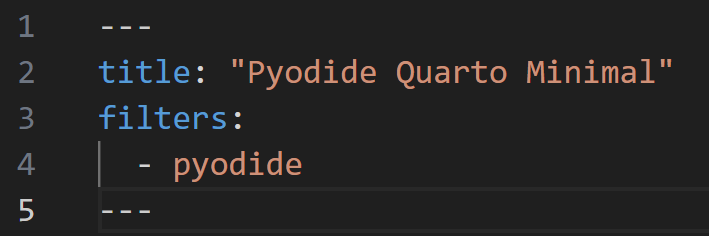
\includegraphics[width=\textwidth]{Images/pyodide_yml_header.png}}
        \end{column}
    \end{columns}
\end{frame}

\begin{frame}{Pyodide-Python in Action}
    \centering
    \fbox{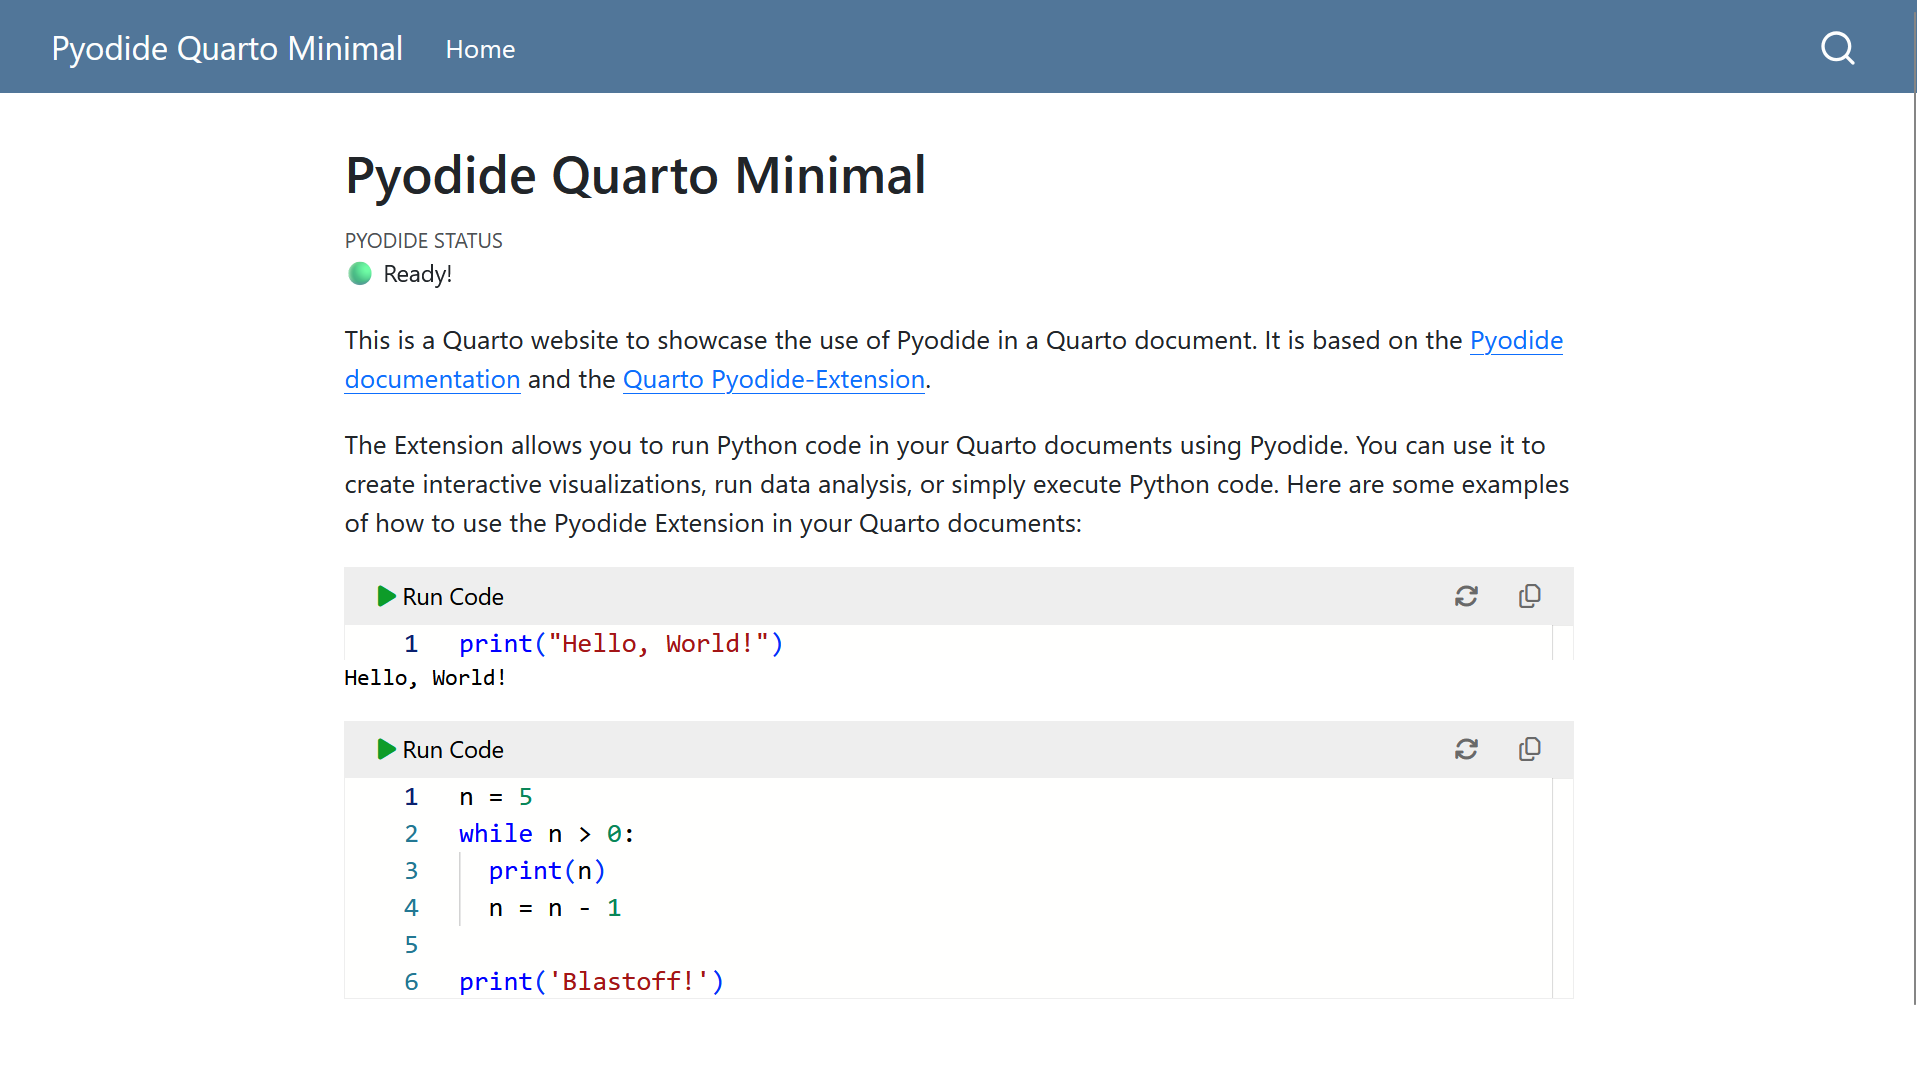
\includegraphics[width=0.7\textwidth, height=0.6\textheight, keepaspectratio]{Images/pyodide_example.png}}

    \vspace{0.5cm}
    \footnotesize A minimal example of a website using the Pyodide-Extension can be found in this repository or directly at: \url{https://gitlab.ruhr-uni-bochum.de/ctm/lund-meeting/-/tree/main/Pyodide\%20Quarto\%20Minimal?ref_type=heads}
\end{frame}

\section{AI-Feedback within Pyodide Python}

\begin{frame}{Pyodide-Python with AI-Feedback}
    \begin{itemize}
        \item At Ruhr University Bochum, we modified the \textbf{coatless-pyodide} extension to include AI feedback.
        \item The extension works the same as the original but adds the ability to ask an AI for help with the code.
        \item To use this feature, users must provide a valid \textbf{API Key} and \textbf{Base URL}.
    \end{itemize}
\end{frame}

\begin{frame}{Pyodide-Python with AI-Feedback in Action}
    \centering
    \fbox{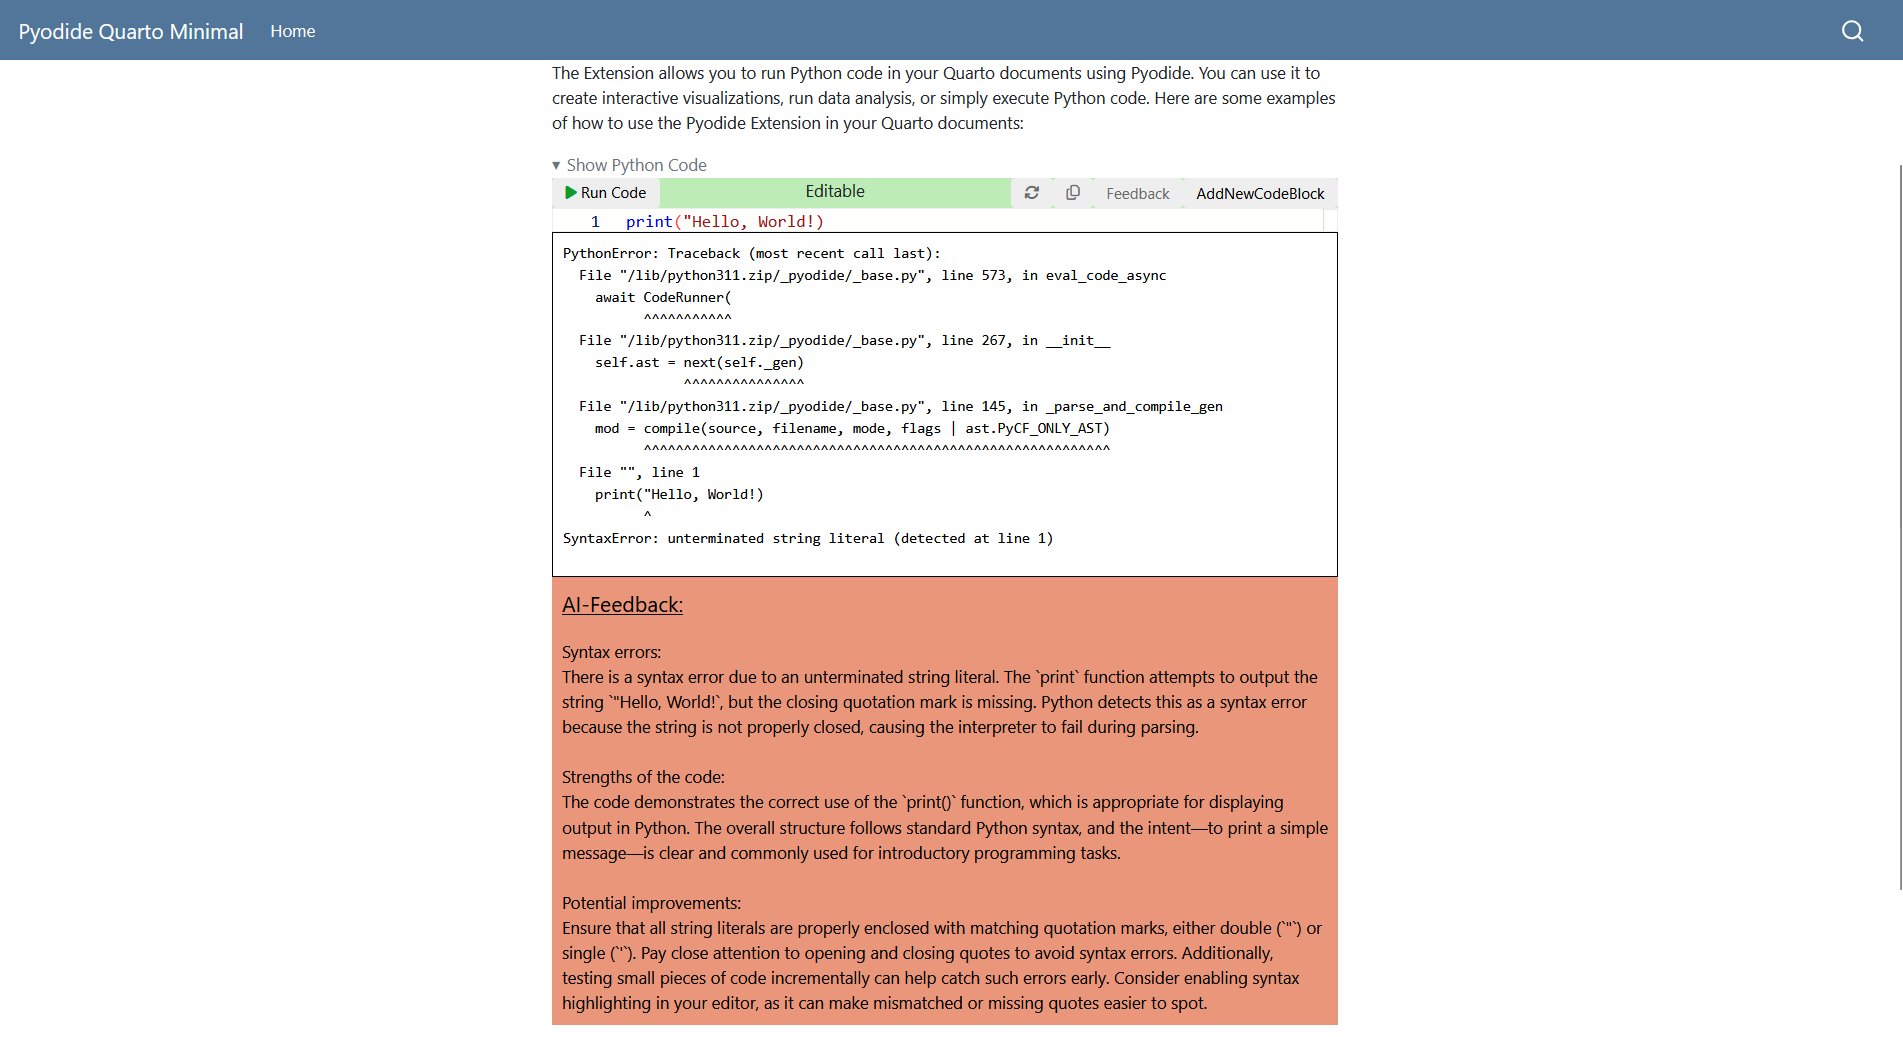
\includegraphics[width=0.7\textwidth, height=0.6\textheight, keepaspectratio]{Images/pyodide_feedback_example.png}}

    \vspace{0.5cm}
    \footnotesize A minimal example of a website using the modified Pyodide-Extension can be found in this repository or directly at: \url{https://gitlab.ruhr-uni-bochum.de/ctm/lund-meeting/-/tree/main/Pyodide-Feedback\%20Minimal?ref_type=heads}
\end{frame}

\section{Quarto Quizzes}

\begin{frame}{Quizdown}
    \begin{itemize}
        \item Gamification can greatly enhance learning, so we wanted to provide a gamified experience in our tutorials.
        \item For this purpose, we looked and found the \textbf{Quizdown} extension: \url{https://github.com/parmsam/quarto-quizdown}
        \item Quizdown allows you to create single-choice, multiple-choice, and ordering quizzes without much extra effort.
    \end{itemize}
\end{frame}

\begin{frame}{Quizdown in Action}
    \centering
    \fbox{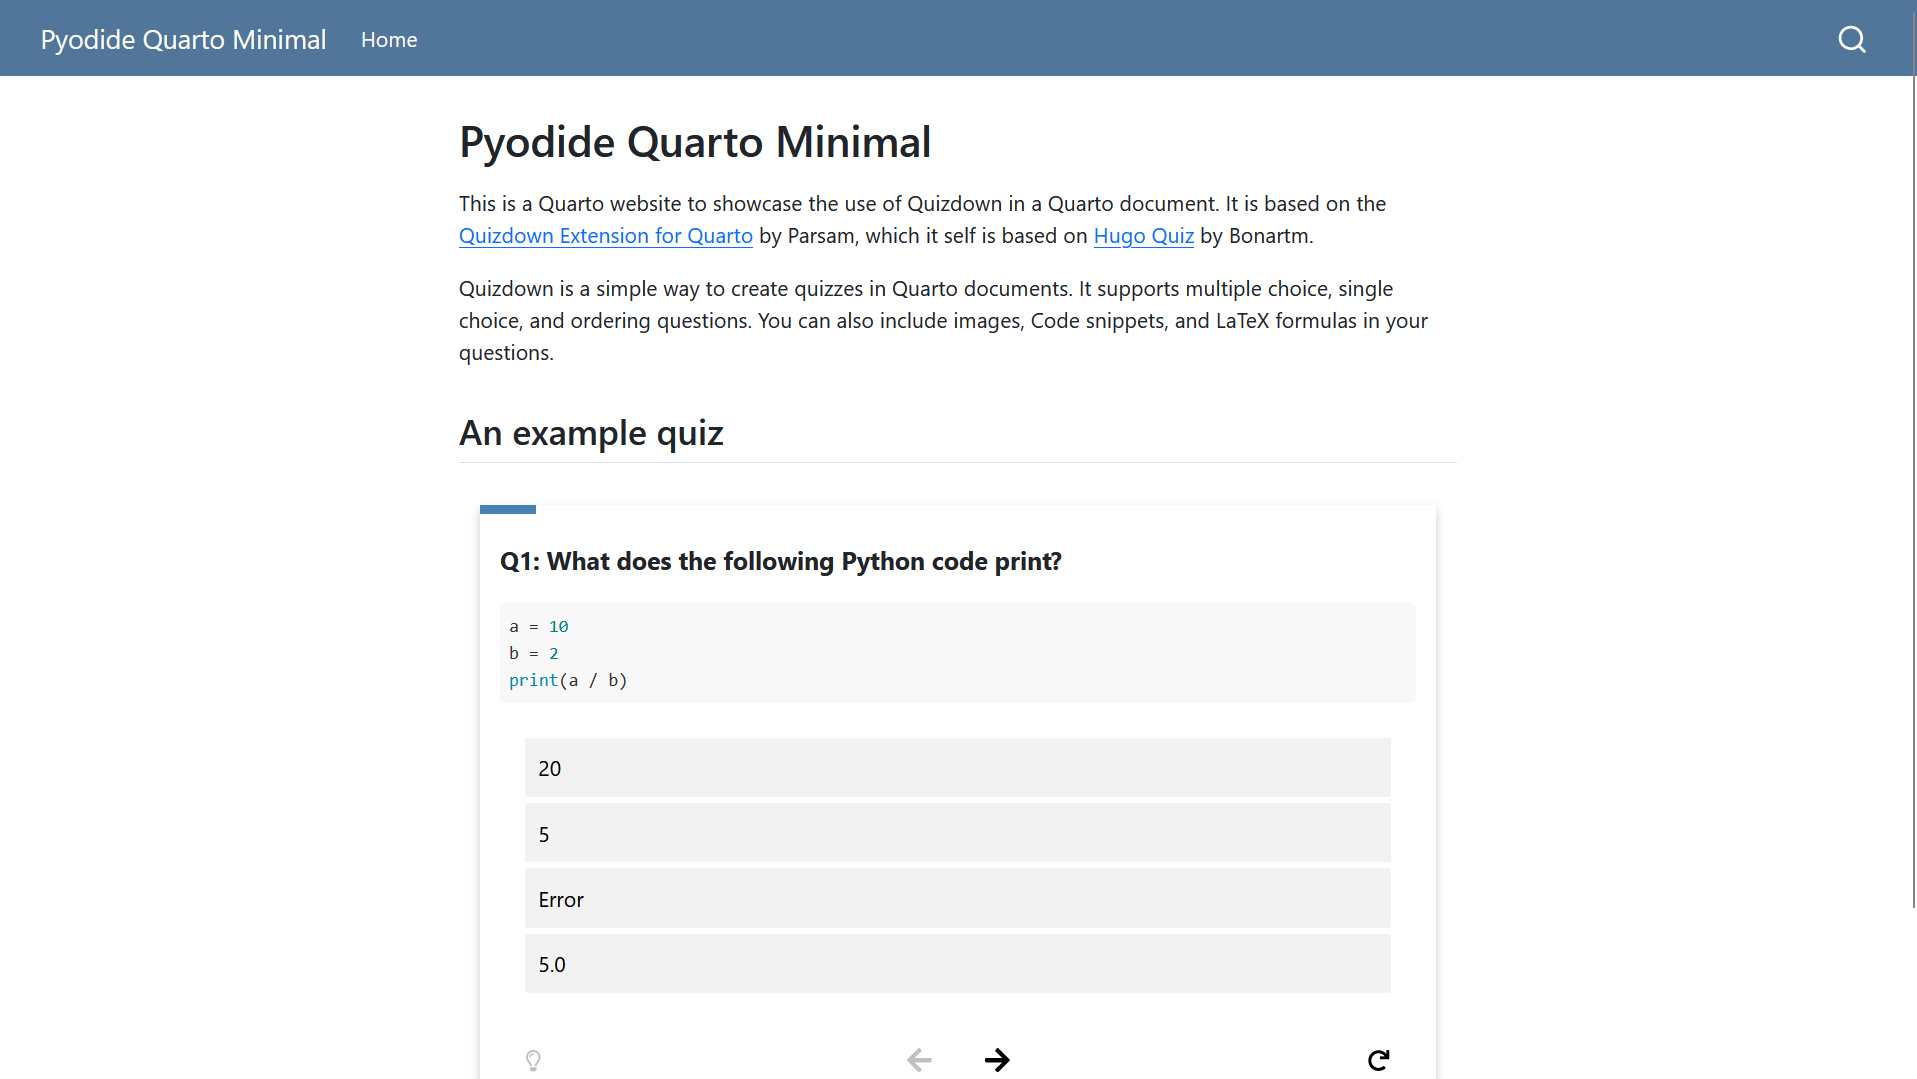
\includegraphics[width=0.7\textwidth, height=0.6\textheight, keepaspectratio]{Images/quizdown_example.png}}

    \vspace{0.5cm}
    \footnotesize A minimal example of a website with Quizdown can be found in this repository or directly at: \url{https://gitlab.ruhr-uni-bochum.de/ctm/lund-meeting/-/tree/main/Quizdown\%20Minimal?ref_type=heads}
\end{frame}

\section {Shinylive}

\begin{frame}{Shinylive}
    \begin{itemize}
        \item In further enhancing the interactive experience we looked for something that would allow us to give users direct feedback on mathematical concepts.
        \item For that we looked into Shiny, specifically the shinylive extension for Quarto: \url{https://github.com/quarto-ext/shinylive}
        \item Shinylive is an extension that lets you embed Shiny apps into your Quarto website.
        \item The app runs entirely in the browser (via WebAssembly), and the code can be edited live with sliders, making the consequences immediately visible.
    \end{itemize}
\end{frame}

\begin{frame}{Shinylive in Action}
    \centering
    \fbox{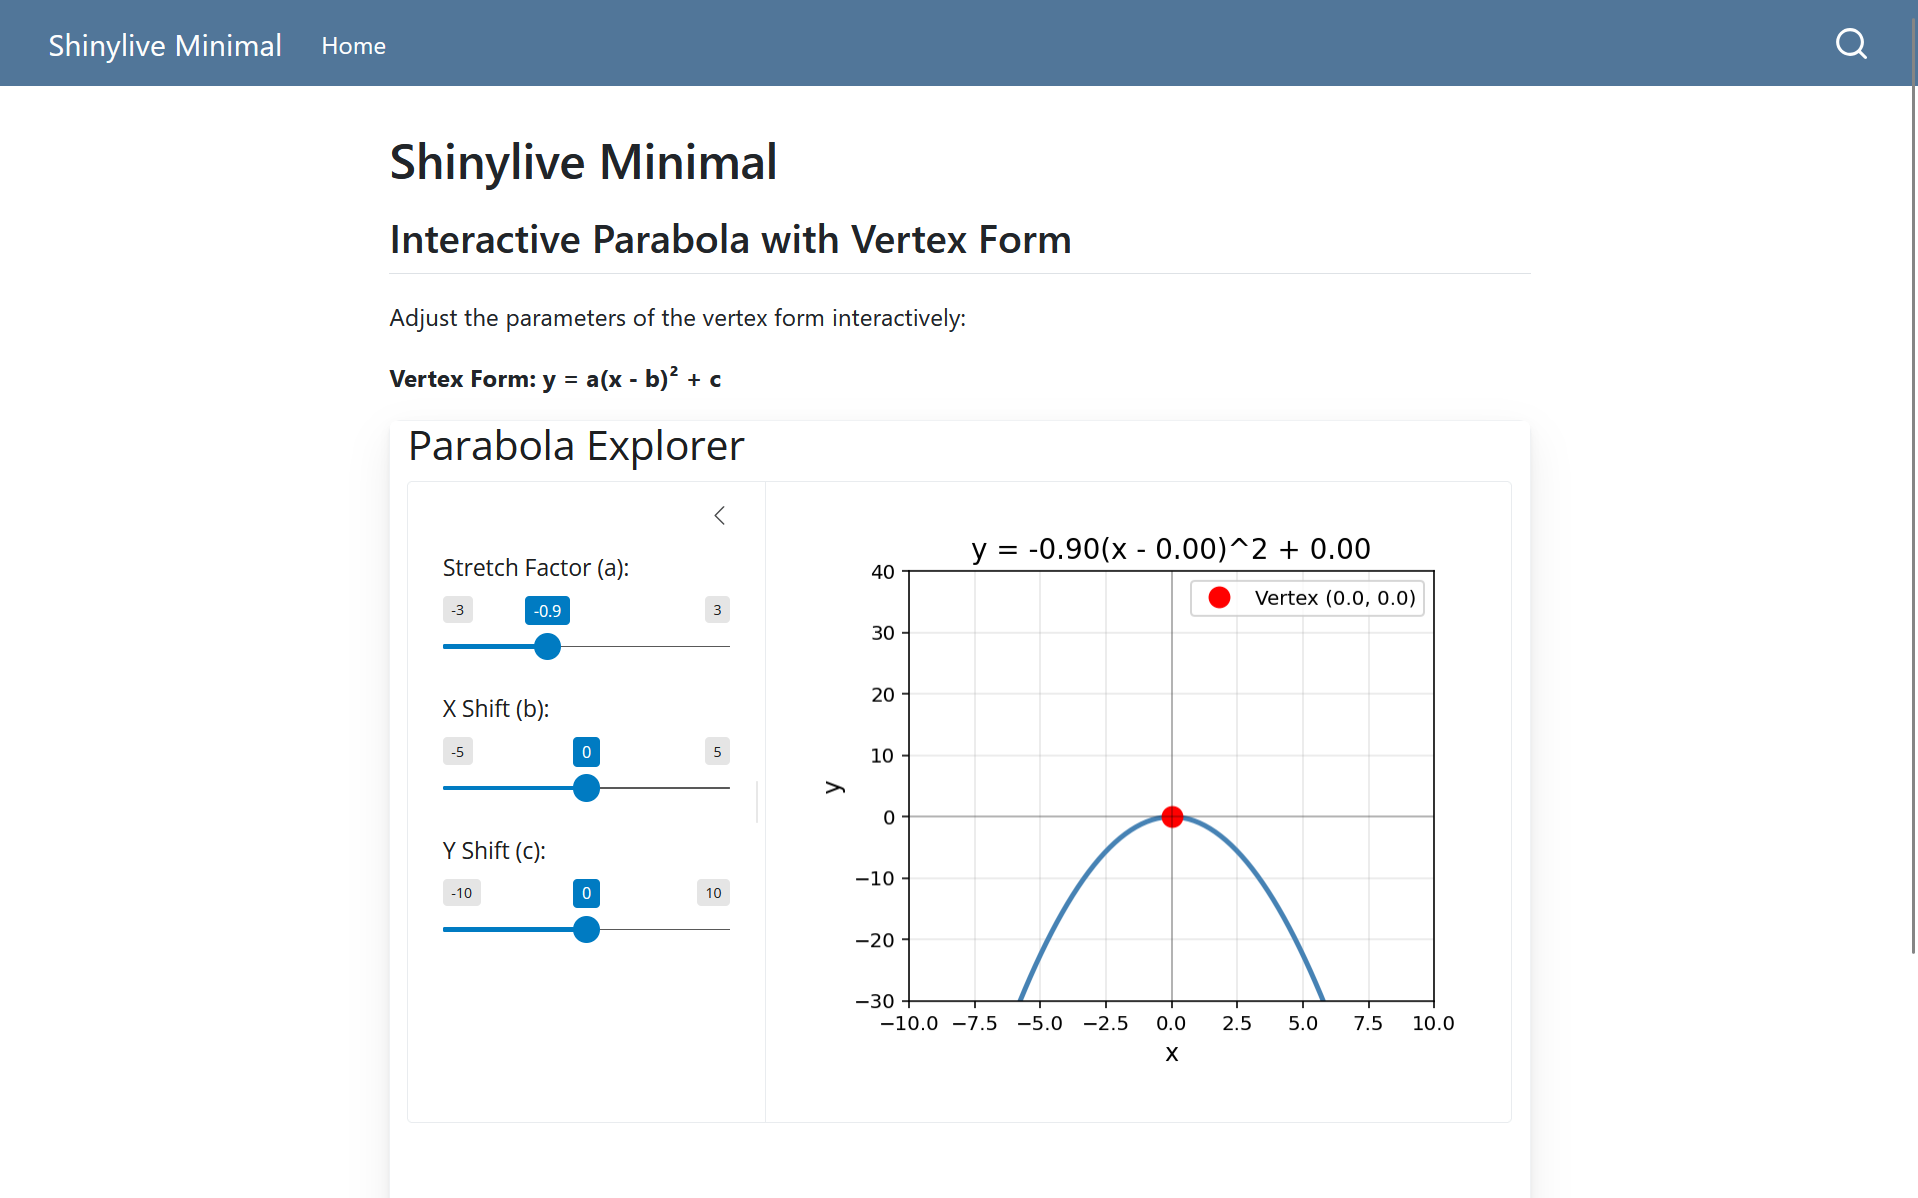
\includegraphics[width=0.7\textwidth, height=0.6\textheight, keepaspectratio]{Images/shinylive_example.png}}

    \vspace{0.5cm}
    \footnotesize A minimal example of a website using the shinylive Extension can be found in this repository or directly at: \url{https://gitlab.ruhr-uni-bochum.de/ctm/lund-meeting/-/tree/main/Shinylive\%20Minimal?ref_type=heads}
\end{frame}
    

\section{Multilanguage Website Projects}

\begin{frame}{Multilanguage Website Projects}
    \begin{itemize}
        \item As this is an international project, we wanted to give users the ability to switch between languages in Quarto.
        \item Currently, there is no official feature to switch languages within a specific part of the website; it only supports redirecting to a different homepage.
        \item Therefore, we wrote a small Python script that modifies the navbar to include a dropdown menu, allowing users to switch languages while staying on the same page.
        \item Quarto's \icode{preview} command does not support the switching between languages, so you won't be able to properly preview your page using \icode{quarto preview}
        \item Instead, run the included Python script to host the site locally and preview it in the browser.
    \end{itemize}
\end{frame}

\begin{frame}{Multilanguage Website Projects in Action}
    \centering
    \fbox{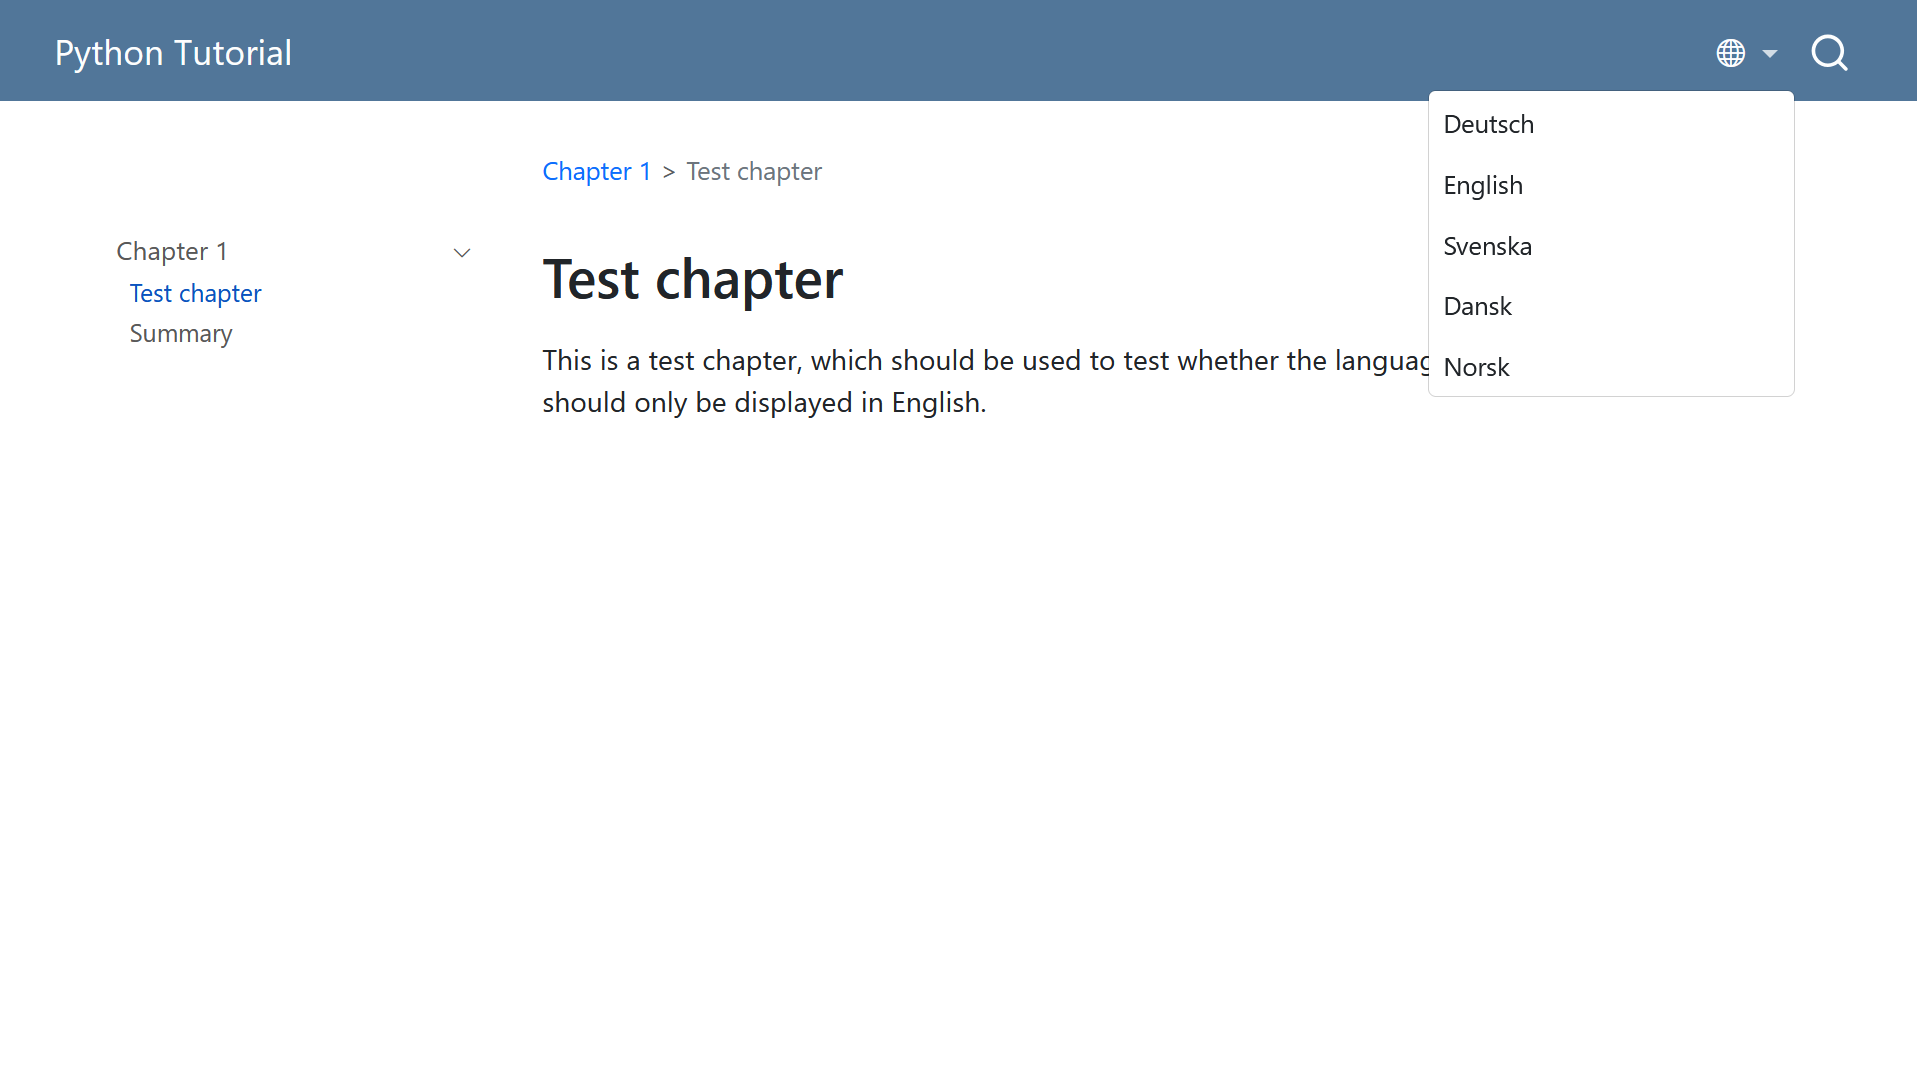
\includegraphics[width=0.7\textwidth, height=0.6\textheight, keepaspectratio]{Images/multilang_example.png}}

    \vspace{0.5cm}
    \footnotesize A minimal example of a website with multi-language support (I hope the AI translations aren't too bad!) can be found in this repository or directly at: \url{https://gitlab.ruhr-uni-bochum.de/ctm/lund-meeting/-/tree/main/Multilanguage\%20Website\%20Setup?ref_type=heads}
\end{frame}

\section{Conclusion}

\begin{frame}{Conclusion}
    \begin{itemize}
        \item Quarto is a powerful tool for creating interactive and engaging educational content, especially in the context of Computational Thinking in Mathematics.
        \item There is a vast number of extensions available, providing many possibilities to enhance the student experience.
        \item As some of you have already seen, Quarto is a user-friendly tool for creating scripts, as it allows you to combine code and output in a single file.
    \end{itemize}
\end{frame}

\begin{frame}{Resources}
    All materials from this presentation and the slides can be found at: \\
    \vspace{0.5cm}
    \url{https://gitlab.ruhr-uni-bochum.de/ctm/lund-meeting}
\end{frame}

\end{document}
